\documentclass[11pt]{article}

\usepackage[margin=1in]{geometry}
\usepackage{amsmath,amssymb,amsthm,mathtools}
\usepackage[authoryear,round]{natbib}
\usepackage{enumitem}
\usepackage{xcolor}
\usepackage{booktabs}
\usepackage{tikz}
\usetikzlibrary{arrows.meta,positioning}
\usepackage[colorlinks=true,linkcolor=blue!50!black,citecolor=blue!50!black,urlcolor=blue!50!black]{hyperref}

\newtheorem{proposition}{Proposition}[section]
\newtheorem{example}[proposition]{Example}
\newtheorem{remark}[proposition]{Remark}
\newtheorem{definition}[proposition]{Definition}

\newcommand{\FL}{\mathbb{F}L}
\newcommand{\dd}[2]{\frac{\partial #1}{\partial #2}}
\newcommand{\R}{\mathbb{R}}

\title{On the Inequivalence of the Formulations of Classical Mechanics}
\author{}
\date{}

\begin{document}

\maketitle

\begin{abstract}
\noindent
The Newtonian, Lagrangian, Hamiltonian, and Hamilton--Jacobi formulations of classical mechanics are routinely presented as equivalent packagings of a single physical theory, related by Hamilton's principle, the Legendre transform, and Jacobi's theorem. This claim is correct, but only under conditions that are rarely stated explicitly and that fail for large, physically important classes of systems. This paper collects and organizes eight distinct ways in which the standard equivalence breaks down: the gap between Hamilton's principle (stationarity of the action) and the popularly stated ``principle of \emph{least} action'' (minimality), which fails beyond a conjugate time fixed by the curvature of the potential and which can be made arbitrarily short; the consequent failure of the boundary-value problem built into Hamilton's principle itself to be well-posed---even for $H=p^2/2m+V(q)$, a sufficiently steep $V$ makes the two-endpoint problem admit no solution, or infinitely many, in contrast to the always-well-posed Newtonian initial-value problem; the existence of singular Lagrangians, for which the Legendre transform is not invertible and Dirac's theory of constraints is required; the divergence, for nonholonomically constrained systems, between the Lagrange--d'Alembert (``nonholonomic'') and variational (``vakonomic'') equations of motion---a disagreement that is empirically decidable rather than merely notational; the existence of Newtonian force laws that admit no Lagrangian description at all, governed by the Helmholtz conditions; the failure of the Legendre transform to be a global diffeomorphism even for pointwise-regular Lagrangians, absent the stronger condition of hyperregularity; the mechanistically identical failure of the Hamilton--Jacobi equation's generating function to stay single-valued beyond a caustic; and an active disagreement in the philosophy of physics literature about whether the Lagrangian and Hamiltonian formulations posit the same geometric structure even where their solution sets coincide exactly. We supply two fully worked examples---a harmonic oscillator exhibiting explicit conjugate points and boundary-value non-uniqueness, and a free particle subject to a simple nonholonomic constraint whose nonholonomic and vakonomic equations of motion are derived explicitly and shown to disagree already at the level of qualitative behavior for identical initial data. We conclude with a short taxonomy distinguishing empirical, mathematical, variational, and structural senses of ``equivalence,'' arguing that no single one of these senses holds uniformly across classical mechanics.
\end{abstract}

\section{Introduction}

Newton's \emph{Principia} (1687) presents mechanics as a theory of forces: bodies possess positions and velocities, forces act on them, and the second law $F = ma$ determines their subsequent motion. A century later, Lagrange's \emph{M\'ecanique analytique} (1788) recast the subject as a variational principle over generalized coordinates---a formulation Lagrange was famously proud to have produced without a single diagram. Half a century after that, Hamilton reformulated Lagrangian mechanics again, trading velocities for momenta via what is now called the Legendre transform and turning the second-order Euler--Lagrange equations into a first-order canonical system on phase space; Jacobi, Poisson, and others quickly extended this into the rich geometric theory of Hamiltonian mechanics. Hamilton went further still, showing that the same dynamics could be extracted from a single first-order partial differential equation for the action itself---the Hamilton--Jacobi equation---a construction Jacobi turned into a practical method for solving Hamiltonian systems by separation of variables.

The pedagogical line ever since has been that these are simply different \emph{formulations} of one and the same physical theory: notational variants, chosen for convenience, that always agree on physical predictions. Textbook treatments typically present the passage between them---d'Alembert's principle on one side, the Legendre transform on the other---as a purely mechanical, always-available translation \citep{goldstein2001,arnold1989}.

This is true, but only inside a restrictive domain that is almost never made explicit: essentially, for systems with holonomic constraints (or none), described by a Lagrangian that is \emph{regular}, and in fact \emph{hyperregular}, if one wants the equivalence to hold globally rather than merely locally. Outside that domain the four formulations can fail to agree in several logically independent ways, some of them merely technical and some of them---most strikingly, in the case of nonholonomic constraints---genuinely physical, in the sense that the different formulations make different, experimentally distinguishable predictions for the same system.

This paper has two aims. First, to collect and organize these failure modes, most of which are individually well known within their own specialist literatures (geometric mechanics, constrained Hamiltonian dynamics, the calculus of variations, philosophy of physics) but rarely assembled in one place. Second, to give a completely worked, self-contained example of the sharpest of these failures---the split between nonholonomic and vakonomic mechanics---so that the disagreement between formulations is visible as explicit, checkable mathematics rather than asserted by citation alone.

Section~\ref{sec:standard} reviews the four standard formulations---Newtonian, Lagrangian, Hamiltonian, and Hamilton--Jacobi---and states the equivalence theorems that license the textbook folklore, making their hypotheses explicit. Section~\ref{sec:failures} works through eight distinct failure modes. Section~\ref{sec:discussion} steps back and asks what ``equivalence'' between formulations of a physical theory ought to mean in the first place, drawing on a debate in the philosophy of physics literature that turns out to be closely tied to the mathematics of Section~\ref{sec:failures}. Section~\ref{sec:conclusion} concludes.

\section{The Four Standard Formulations}
\label{sec:standard}

\subsection{Newtonian mechanics}

For a system of $N$ particles with positions $\mathbf{r}_i \in \R^3$, Newton's second law reads $m_i \ddot{\mathbf{r}}_i = \mathbf{F}_i$, where $\mathbf{F}_i$ is the total force on particle $i$. Constraints are handled by splitting the force into an applied part and a constraint (reaction) part, $\mathbf{F}_i = \mathbf{F}_i^{\mathrm{app}} + \mathbf{F}_i^{\mathrm{c}}$, and postulating---this is d'Alembert's principle---that the constraint forces do no virtual work: $\sum_i \mathbf{F}_i^{\mathrm{c}}\cdot \delta \mathbf{r}_i = 0$ for every virtual displacement $\delta\mathbf{r}_i$ compatible with the constraints at a frozen instant of time. It is d'Alembert's principle, not Newton's second law by itself, that supplies the bridge to the variational formulations below; as we will see in Section~\ref{sec:nonholonomic}, exactly how one operationalizes ``compatible with the constraints'' is where nonholonomic constraints cause trouble.

\subsection{Lagrangian mechanics}

Let $Q$ be the configuration manifold and $TQ$ its tangent bundle, with induced coordinates $(q^i,\dot q^i)$. A Lagrangian is a function $L : TQ \times \R \to \R$, typically (but not necessarily) of the form $L = T - V$, kinetic minus potential energy. Hamilton's principle asserts that physical trajectories $q(t)$ extremize the action
\begin{equation}
S[q(\cdot)] = \int_{t_0}^{t_1} L\big(q(t),\dot q(t), t\big)\, dt
\end{equation}
among curves with fixed endpoints $q(t_0), q(t_1)$. Setting the first variation to zero yields the Euler--Lagrange equations
\begin{equation}
\label{eq:EL}
\frac{d}{dt}\dd{L}{\dot q^i} - \dd{L}{q^i} = 0 , \qquad i = 1,\dots,n=\dim Q .
\end{equation}
For a system subject to \emph{ideal, holonomic} constraints, this is fully equivalent to Newton's second law plus d'Alembert's principle, once $Q$ is taken to be the constraint surface itself and the $q^i$ are independent generalized coordinates on it.

\subsection{Hamiltonian mechanics}

Define the momenta $p_i = \partial L/\partial \dot q^i$. This is the \emph{fiber derivative} $\FL: TQ \to T^*Q$, $(q,\dot q)\mapsto (q,p)$. Where $\FL$ can be inverted for $\dot q$ in terms of $(q,p)$, one defines the Hamiltonian by the Legendre transform,
\begin{equation}
H(q,p,t) = p_i \dot q^i - L(q,\dot q, t)\Big|_{\dot q = \dot q(q,p,t)} ,
\end{equation}
and Hamilton's canonical equations
\begin{equation}
\label{eq:Ham}
\dot q^i = \dd{H}{p_i}, \qquad \dot p_i = -\dd{H}{q^i}
\end{equation}
reproduce~\eqref{eq:EL} on the nose. The cotangent bundle $T^*Q$ carries a canonical symplectic form $\omega = dp_i \wedge dq^i$, giving Hamiltonian mechanics its distinctive geometry: canonical transformations, Poisson brackets, Liouville's theorem, and so on.

\subsection{The standard equivalence theorem, and its silent hypotheses}
\label{sec:hypotheses}

The precise statement licensing the textbook claim is the following.

\begin{proposition}[Regular equivalence]
\label{prop:regular}
Let $L: TQ\times\R\to\R$ be \emph{regular}: the fiber Hessian $W_{ij} = \partial^2 L/\partial \dot q^i \partial \dot q^j$ is nondegenerate at every point of $TQ$. Then $\FL$ is a local diffeomorphism, $H$ is well defined locally, and solutions of~\eqref{eq:EL} correspond, via $p = \FL(q,\dot q)$, bijectively and locally to solutions of~\eqref{eq:Ham}. If in addition $\FL$ is a \emph{global} diffeomorphism $TQ \to T^*Q$---in which case $L$ is called \emph{hyperregular}---this correspondence extends to a global bijection between the full solution spaces of the two theories \citep{abrahammarsden}.
\end{proposition}

\subsection{Hamilton--Jacobi theory}
\label{sec:hjtheory}

A fourth formulation, historically inseparable from Hamilton's own work, replaces the $2n$ first-order equations~\eqref{eq:Ham} by a single first-order partial differential equation for a scalar function. Define \emph{Hamilton's principal function} $S(q,t)$ as the action evaluated along the true trajectory of the system that starts at some fixed reference event $(q_0,t_0)$ and ends at $(q,t)$. Hamilton showed that, viewed as a function of its endpoint, $S$ satisfies the \emph{Hamilton--Jacobi equation}
\begin{equation}
\label{eq:HJ}
\dd{S}{t} + H\Big(q,\dd{S}{q},t\Big) = 0 .
\end{equation}
Conversely, Jacobi showed how to run this construction backwards and recover the canonical equations~\eqref{eq:Ham} directly from~\eqref{eq:HJ}, without integrating an ordinary differential equation, provided one can find a \emph{complete integral}: an $n$-parameter family of solutions $S(q,t;\alpha)$, $\alpha=(\alpha_1,\dots,\alpha_n)$, of~\eqref{eq:HJ} whose mixed Hessian $\partial^2 S/\partial q^i\partial \alpha_j$ is everywhere nondegenerate on the domain of interest.

\begin{proposition}[Jacobi's theorem]
\label{prop:jacobi-thm}
Let $S(q,t;\alpha)$ be a complete integral of~\eqref{eq:HJ} on an open set $U\subset Q\times\R$, with $\det(\partial^2 S/\partial q^i\partial\alpha_j)\neq 0$ throughout $U$. Then the equations
\begin{equation}
\dd{S}{\alpha_j} = \beta_j \ (\text{constants}), \qquad p_i = \dd{S}{q^i}
\end{equation}
implicitly define, for each choice of constants $(\alpha,\beta)$, a curve $(q(t),p(t))$ solving Hamilton's equations~\eqref{eq:Ham} on $U$; every solution of~\eqref{eq:Ham} passing through $U$ arises this way for a suitable choice of $(\alpha,\beta)$ \citep{arnold1989,goldstein2001}.
\end{proposition}

Proposition~\ref{prop:jacobi-thm} is the formal engine behind solving Hamiltonian systems by separation of variables, and it is a genuine equivalence result: wherever a complete integral with nondegenerate mixed Hessian exists, the Hamilton--Jacobi and Hamiltonian pictures determine exactly the same trajectories. The qualification ``on the domain of interest'' is doing real work, however---Section~\ref{sec:caustics} shows that it cannot in general be dropped, and that its failure is tied to the same mechanism that undermines the ``least action'' reading of Hamilton's principle in Section~\ref{sec:jacobi}.

Everything that follows in Section~\ref{sec:failures} concerns ways in which the hypotheses of Proposition~\ref{prop:regular} or Proposition~\ref{prop:jacobi-thm} can fail to hold, or ways in which their being satisfied does not settle every reasonable sense in which one might want two physical theories to be ``the same.'' Table~\ref{tab:summary} previews the eight failure modes and where each one sits relative to these two propositions.

\begin{table}[htbp]
\centering
\small
\begin{tabular}{@{}p{2.6cm}p{4.4cm}p{5.6cm}@{}}
\toprule
\textbf{Comparison} & \textbf{Condition needed for equivalence} & \textbf{What happens when it fails} \\
\midrule
Hamilton's principle $\leftrightarrow$ least action & Trajectory ends before the first conjugate point & Action is a saddle point, not a minimum, past a conjugate point (\S\ref{sec:jacobi}) \\
Newtonian (initial-value) $\leftrightarrow$ Hamilton's principle (boundary-value) & Travel time less than the first conjugate time & Boundary-value problem may have no solution or infinitely many (\S\ref{sec:bvp}) \\
Newtonian $\leftrightarrow$ Lagrangian & Force law satisfies the Helmholtz self-adjointness conditions & No Lagrangian exists at all (\S\ref{sec:helmholtz}) \\
Lagrangian (unconstrained) $\leftrightarrow$ Lagrangian under nonholonomic constraints & --- constraint type is itself the fork & Lagrange--d'Alembert and vakonomic mechanics diverge (\S\ref{sec:nonholonomic}) \\
Lagrangian $\leftrightarrow$ Hamiltonian (local) & $L$ regular (nondegenerate fiber Hessian) & Dirac's constraint algorithm required (\S\ref{sec:singular}) \\
Lagrangian $\leftrightarrow$ Hamiltonian (global) & $L$ hyperregular ($\FL$ a global diffeomorphism) & $\FL$ fails to be onto or one-to-one globally (\S\ref{sec:global}) \\
Hamiltonian $\leftrightarrow$ Hamilton--Jacobi & Complete integral exists with nondegenerate mixed Hessian & Generating function becomes multivalued at a caustic (\S\ref{sec:caustics}) \\
``The same'' system, different representatives & --- & Gauge freedom: many Lagrangians/Hamiltonians per force law (\S\ref{sec:nonunique}) \\
\bottomrule
\end{tabular}
\caption{The eight failure modes discussed in Section~\ref{sec:failures}, and where each sits relative to the regular equivalence theorem (Proposition~\ref{prop:regular}) or Jacobi's theorem (Proposition~\ref{prop:jacobi-thm}).}
\label{tab:summary}
\end{table}

Figure~\ref{fig:map} maps the Newtonian--Lagrangian--Hamiltonian chain specifically, with the corresponding points of failure marked; the three further failure modes concerning the variational character of the action, the well-posedness of its boundary-value problem, and the global validity of the Hamilton--Jacobi correspondence (\S\ref{sec:jacobi}, \S\ref{sec:bvp}, \S\ref{sec:caustics}) are internal to the Lagrangian and Hamiltonian formulations respectively and are not separately diagrammed.

\begin{figure}[htbp]
\centering
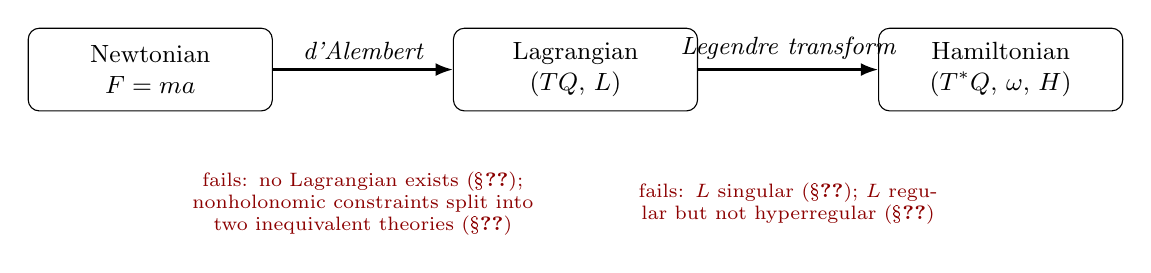
\begin{tikzpicture}[
    box/.style={draw, rounded corners, minimum width=3.1cm, minimum height=1.05cm, align=center, font=\small},
    lbl/.style={font=\scriptsize, align=center, text width=4.6cm, text=red!55!black}
]
\node[box] (N) at (0,0)   {Newtonian\\ $F=ma$};
\node[box] (L) at (5.4,0) {Lagrangian\\ $(TQ,\,L)$};
\node[box] (H) at (10.8,0){Hamiltonian\\ $(T^*Q,\,\omega,\,H)$};

\draw[-{Latex[length=2.2mm]}, thick] (N) -- (L) node[midway, above, font=\small\itshape] {d'Alembert};
\draw[-{Latex[length=2.2mm]}, thick] (L) -- (H) node[midway, above, font=\small\itshape] {Legendre transform};

\node[lbl] at (2.7,-1.7) {fails: no Lagrangian exists (\S\ref{sec:helmholtz}); nonholonomic constraints split into two inequivalent theories (\S\ref{sec:nonholonomic})};
\node[lbl] at (8.1,-1.7) {fails: $L$ singular (\S\ref{sec:singular}); $L$ regular but not hyperregular (\S\ref{sec:global})};
\end{tikzpicture}
\caption{The standard chain of formulations, annotated with the conditions under which each arrow fails to deliver an equivalence.}
\label{fig:map}
\end{figure}

\section{Where Exact Equivalence Fails}
\label{sec:failures}

\subsection{Extremal versus minimal: Jacobi's conjugate-point theorem}
\label{sec:jacobi}

The equivalence between Hamilton's principle and the Euler--Lagrange equations~\eqref{eq:EL} is exact and unconditional: $\delta S=0$ for all admissible variations if and only if~\eqref{eq:EL} holds along the trajectory. This is a first-order, local statement about the action, and none of Section~\ref{sec:standard} depends on anything more. But the popular name for Hamilton's principle---the ``principle of \emph{least} action''---asserts something stronger: that the true trajectory does not merely make $S$ stationary but \emph{minimizes} it among nearby competitors with the same endpoints. This stronger claim concerns the second variation, not the first, and it is generally false, even for the most elementary holonomic, unconstrained, regular Lagrangian system one could write down \citep{gray2009,graytaylor2007}.

For a one-dimensional natural Lagrangian $L(x,\dot x) = \tfrac12 m\dot x^2 - V(x)$, consider a perturbation $x(t)+\varepsilon\eta(t)$ of a solution $x(t)$ of~\eqref{eq:EL}, with $\eta(t_0)=\eta(t_1)=0$. The second variation of the action is
\begin{equation}
\delta^2 S[\eta] = \int_{t_0}^{t_1} \Big[ m\dot\eta(t)^2 - V''(x(t))\,\eta(t)^2 \Big]\, dt ,
\end{equation}
and the trajectory is a genuine local minimum of $S$ if and only if $\delta^2S[\eta]>0$ for every admissible $\eta\not\equiv0$. Whether this holds is governed by the \emph{Jacobi accessory equation}, obtained by linearizing~\eqref{eq:EL} about $x(t)$,
\begin{equation}
\label{eq:jacobi-eq}
m\ddot\eta + V''(x(t))\,\eta = 0 ,
\end{equation}
together with $\eta(t_0)=0$. A time $t_c>t_0$ is a \emph{conjugate point} (or \emph{kinetic focus}) to $t_0$ along the trajectory if the nontrivial solution of~\eqref{eq:jacobi-eq} with $\eta(t_0)=0$ vanishes again at $t_c$.

\begin{proposition}[Jacobi's necessary condition]
\label{prop:jacobi-necessary}
The trajectory $x(t)$ furnishes a local minimum of the action on $[t_0,t_1]$ only if $t_1$ occurs before the first conjugate point to $t_0$. If $t_1$ lies beyond the first conjugate point, $S$ is a saddle point at $x(t)$: nearby trial trajectories exist with strictly smaller action, even though $x(t)$ exactly satisfies~\eqref{eq:EL} \citep{gelfandfomin1963,gray2009}.
\end{proposition}

\begin{example}[Harmonic oscillator]
\label{ex:sho}
Take $V(x)=\tfrac12 kx^2$, so $V''\equiv k$ and~\eqref{eq:jacobi-eq} becomes $\ddot\eta+\omega^2\eta=0$ with $\omega=\sqrt{k/m}$. The solution with $\eta(t_0)=0$ is $\eta(t)=\sin\!\big(\omega(t-t_0)\big)$, which next vanishes at $t_c=t_0+\pi/\omega$---exactly half a period. By Proposition~\ref{prop:jacobi-necessary}, a segment of oscillator trajectory genuinely minimizes the action if its duration is less than $\pi/\omega$, and is merely a stationary saddle point if its duration exceeds $\pi/\omega$.
\end{example}

Example~\ref{ex:sho} answers, quantitatively, the question of how short is ``short enough.'' The conjugate-point time $\pi/\omega=\pi\sqrt{m/k}$ is set entirely by the curvature $V''=k$ of the potential and shrinks without bound as $k$ grows: no fixed time interval is safe for every system, because a sufficiently steeply curved potential will already have produced a conjugate point within it. More generally, conjugate points arise only where $V''>0$ along the trajectory; for potentials with $V''(x)\leq 0$ for all $x$ (a free particle, uniform gravity, an inverted quadratic barrier) no conjugate point ever forms, and the action is minimized for arbitrarily long times \citep{gray2009}. Whether ``the action is minimized'' is therefore not a property of Hamilton's principle in general---it is a property of the specific potential, and specifically of how sharply it curves.

It is worth being precise about what this does and does not show. Hamilton's principle, in its correct form ($\delta S=0$), remains exactly equivalent to Newton's second law throughout; nothing here contradicts Proposition~\ref{prop:regular}. What fails is the stronger, popularly stated identification of Hamilton's principle with a principle of \emph{least} action---and it fails already in the cleanest setting available anywhere in this paper: a single unconstrained particle, regular and hyperregular Lagrangian, smooth potential. That is precisely why this failure mode belongs at the head of this section, ahead of the more exotic constructions that follow.

\subsection{Non-existence and non-uniqueness: the boundary-value problem}
\label{sec:bvp}

Section~\ref{sec:jacobi} asked whether a trajectory already known to satisfy~\eqref{eq:EL} minimizes the action. A logically prior question is whether such a trajectory exists and is unique at all, given the data Hamilton's principle is actually stated in terms of: not an initial position and velocity, but two fixed \emph{endpoints}, $q(t_0)=q_A$ and $q(t_1)=q_B$---exactly the boundary conditions built into the action functional in Section~\ref{sec:standard}. This is a fundamentally different mathematical problem from the Newtonian initial-value problem. Given $(q_0,\dot q_0)$ at a single instant, standard ODE theory (Picard--Lindelöf) guarantees a unique solution of~\eqref{eq:EL}, at least locally in time, for any reasonably smooth force law: the ``most boring'' Hamiltonian, $H=p^2/2m+V(q)$, is always well-posed as an initial-value problem. Fixing $q(t_0)$ and $q(t_1)$ instead offers no such guarantee. The boundary-value problem can have no solution, a unique solution, or infinitely many, and which of these holds is governed by exactly the conjugate points of Section~\ref{sec:jacobi}.

Fix $t_0$ and $q_A=q(t_0)$, and let $x(t,v_0)$ denote the unique initial-value solution with $\dot x(t_0)=v_0$. The \emph{shooting map} $v_0\mapsto x(t_1,v_0)$ determines which endpoints are reachable in time $T=t_1-t_0$ and how many initial velocities reach a given one. Its derivative $\partial x(t,v_0)/\partial v_0$ satisfies~\eqref{eq:EL} linearized about the trajectory---for $H=p^2/2m+V(q)$ this is exactly the Jacobi accessory equation~\eqref{eq:jacobi-eq}, with initial data $\eta(t_0)=0$, $\dot\eta(t_0)=1$. Consequently
\begin{equation}
\dd{x(t_1,v_0)}{v_0} = 0 \quad\Longleftrightarrow\quad t_1 \text{ is a conjugate point to } t_0 ,
\end{equation}
so the shooting map is a local diffeomorphism precisely up to the first conjugate time, and can fold---losing injectivity, surjectivity, or both---at and beyond it.

\begin{example}[Harmonic oscillator boundary-value problem]
\label{ex:sho-bvp}
Continuing Example~\ref{ex:sho}, set $t_0=0$, $q_A=0$. The initial-value solution is $x(t,v_0)=(v_0/\omega)\sin(\omega t)$, so the shooting map to time $T$ is $v_0\mapsto (v_0/\omega)\sin(\omega T)$, and
\begin{equation}
v_0 = \frac{\omega\, q_B}{\sin(\omega T)}
\end{equation}
solves $x(0)=0$, $x(T)=q_B$ whenever $\sin(\omega T)\neq0$: a unique solution, as expected for $T$ short of the first conjugate time $\pi/\omega$. But at $T=n\pi/\omega$ for a positive integer $n$---an integer multiple of the conjugate time---$\sin(\omega T)=0$ identically, and the shooting map collapses to $v_0\mapsto 0$ regardless of $v_0$: for $q_B\neq0$ \emph{no} solution exists, while for $q_B=0$ \emph{every} $v_0\in\R$ solves the boundary-value problem, a one-parameter family of distinct true trajectories connecting the same two events \citep{gray2009}.
\end{example}

Example~\ref{ex:sho-bvp} shows non-existence and non-uniqueness sitting on opposite sides of the same coincidence, both triggered by the same conjugate-time condition, and both occurring for the most elementary confining potential there is. The critical travel times $n\pi/\omega$ are evenly spaced only because the harmonic oscillator's own equation of motion is already linear---so it coincides with its own Jacobi equation, and conjugate points recur exactly periodically. For a general potential, the accessory equation~\eqref{eq:jacobi-eq} has a time-varying coefficient $V''(x(t))/m$ and the conjugate times need not be evenly spaced, but the qualitative picture survives, and can be more dramatic still: \citet{gray2009} exhibits a quartic oscillator, $V(x)=\tfrac14 Cx^4$, in which a whole family of distinct true trajectories leaving a common starting event recross one another at a common later event, producing multiple genuinely different---not merely differently scaled---solutions of the same boundary-value problem.

The dependence on how fast the potential curves is exactly the one identified in Section~\ref{sec:jacobi}: since $\omega=\sqrt{k/m}$ for the harmonic case, the critical travel times $n\pi/\omega = n\pi\sqrt{m/k}$ shrink as the curvature $k$ grows, so for \emph{any} fixed travel time $T$, a steep enough potential well places $T$ at or past a degenerate configuration. ``The most boring system there is,'' $H=p^2/2m+V(q)$, therefore fails to have a well-posed boundary-value problem in exactly the regime---strongly confining, rapidly growing $V$---that most textbook potentials are drawn from.

This multiplicity is not a curiosity confined to classical mechanics: it is exactly what the Feynman path-integral formulation of quantum mechanics must sum over. The semiclassical propagator between $q_A$ and $q_B$ is, in general, a sum of contributions from \emph{every} classical trajectory solving the boundary-value problem, each carrying a phase determined by its action together with a further phase set by the \emph{Maslov index}---the number of conjugate points the trajectory has crossed \citep{gray2009}. The Maslov index is, in this sense, a bookkeeping device for exactly the multiplicity established in this section: it is needed because the classical boundary-value problem it quantizes is not, in general, uniquely solvable.

\subsection{Singular Lagrangians and constrained Hamiltonian dynamics}
\label{sec:singular}

A Lagrangian is \emph{singular} (or degenerate) when its fiber Hessian $W_{ij} = \partial^2 L/\partial \dot q^i \partial \dot q^j$ is degenerate somewhere on $TQ$. In that case $\FL$ is not a local diffeomorphism there: the momenta $p_i = \partial L/\partial \dot q^i$ are not independent functions of the velocities, and one cannot solve for all of $\dot q$ in terms of $(q,p)$. Concretely, degeneracy of $W_{ij}$ means the map $\FL$ satisfies one or more relations
\begin{equation}
\phi_a(q,p) = 0, \qquad a = 1,\dots,k,
\end{equation}
purely among the momenta and coordinates---\emph{primary constraints}, in Dirac's terminology---that hold identically on the image of $\FL$, before any equations of motion are imposed.

The cleanest illustration is to note that Hamiltonian mechanics is itself, formally, a maximally singular special case of Lagrangian mechanics. Treat $(q,p)$ as $2n$ independent coordinates on an auxiliary configuration space and consider the first-order ``Hamiltonian-form'' Lagrangian
\begin{equation}
L_1(q,p,\dot q,\dot p) = p_i \dot q^i - H(q,p).
\end{equation}
Its Euler--Lagrange equations reproduce~\eqref{eq:Ham} exactly, so in one sense Hamiltonian mechanics \emph{is} a special case of Lagrangian mechanics on a bigger space. But the fiber Hessian of $L_1$ with respect to $(\dot q,\dot p)$ vanishes identically---$L_1$ is linear, not quadratic, in the velocities---so $L_1$ is about as singular as a Lagrangian can be, and the naive Legendre-transform machinery of Section~\ref{sec:hypotheses} simply does not apply to it. Recovering Hamilton's equations from $L_1$ requires running the full constrained-Hamiltonian algorithm below, not the regular Legendre transform.

The general treatment of singular Lagrangians is due to Dirac and Bergmann \citep{dirac1964}. One passes to the \emph{primary constraint surface} $\Sigma_1 \subset T^*Q$ cut out by the $\phi_a$, and checks whether the primary constraints are preserved under time evolution generated by a (now only partially determined) Hamiltonian; if not, this consistency requirement generates \emph{secondary constraints}, and the process is iterated until a stable constraint surface is reached. Constraints are further classified as \emph{first class} (those with vanishing Poisson brackets with all other constraints, which typically signal gauge freedom---directions in phase space that are not physically distinguishable) or \emph{second class} (which can be eliminated using the Dirac bracket, an amended Poisson bracket adapted to the constraint surface) \citep{henneauxteitelboim1992}. The upshot is that for a singular $L$, the physical phase space is not $T^*Q$ but a further-reduced submanifold, of dimension strictly smaller than $2n$ in the presence of first-class constraints, and the map from Lagrangian solutions to Hamiltonian solutions is not the clean bijection of Proposition~\ref{prop:regular} but a considerably more elaborate correspondence, often carrying residual gauge freedom on the Lagrangian side that has no counterpart in a naively written-down Hamiltonian system.

Singular Lagrangians are not a pathology confined to toy examples: they are the generic situation for gauge theories. Electromagnetism, Yang--Mills theory, and general relativity all have singular Lagrangians, precisely because the local gauge symmetry (arising from Noether's second theorem) forces degeneracy of the fiber Hessian. For essentially all of fundamental field theory, then, the ``equivalence'' between the Lagrangian and Hamiltonian pictures is not the elementary Legendre-transform story of Section~\ref{sec:hypotheses} at all, but the considerably more delicate Dirac--Bergmann correspondence.

\subsection{Nonholonomic constraints: Lagrange--d'Alembert versus vakonomic mechanics}
\label{sec:nonholonomic}

The sharpest failure of equivalence---sharp enough to be settled experimentally rather than merely by definitional fiat---occurs already at the level of the passage from Newtonian to Lagrangian mechanics, once the constraints are \emph{nonholonomic}: constraints on velocities that cannot be integrated to constraints on configuration alone. The rolling of a coin or a ball without slipping is the standard example.

For holonomic constraints there is no ambiguity in how to build a variational principle: one simply restricts the configuration space $Q$ to the constraint surface and applies Hamilton's principle there. For nonholonomic constraints, given as a distribution $\mathcal{D}\subset TQ$ (a smoothly varying subspace of admissible velocities), there turn out to be two inequivalent ways to generalize the construction, and classical mechanics contains no a priori argument for preferring one over the other on variational grounds alone:

\begin{itemize}[leftmargin=1.4em]
\item \textbf{Nonholonomic (Lagrange--d'Alembert) mechanics.} One directly generalizes d'Alembert's principle: the physical trajectory satisfies the constraint at every instant, and virtual displacements $\delta q$ used in varying the action are required to lie in $\mathcal{D}$ pointwise along the trajectory, \emph{without} imposing the constraint as a restriction on the class of curves being compared. This is the classical, and---as discussed below---experimentally correct, treatment.
\item \textbf{Vakonomic mechanics.} (The name, coined by Kozlov, abbreviates ``variational axiomatic kind'' of mechanics; \citealp{kozlov1983,akn2006}.) One instead builds the constraint directly into the variational problem, extremizing the action over the class of curves that satisfy the constraint at every instant, in the ordinary sense of a constrained extremum problem (formally, via a Lagrange multiplier function adjoined to the Lagrangian).
\end{itemize}

These two constructions look superficially similar---both are ``variational'' and both use Lagrange multipliers to enforce the same constraint---but they generically yield \emph{different} equations of motion for the same Lagrangian and the same constraint. \citet{lewismurray1995} worked this comparison out in detail for a ball rolling without slipping on a rotating table, deriving both sets of equations and testing each against a physical experiment; they found good agreement between the nonholonomic equations (once realistic friction is included) and the observed motion, and were unable to reproduce the observations with the vakonomic equations. The nonholonomic/vakonomic split is accordingly not a matter of taste or convenience: it is a case in which two ways of extending the Lagrangian formalism to a wider class of systems make different, checkable predictions, and only one of them is the physically correct generalization of Newtonian mechanics with ideal constraint forces \citep{neimarkfufaev1972,bloch2003}.

\subsubsection{A fully worked example}

To make the disagreement completely explicit, consider the simplest possible illustration: a free particle of unit mass in $Q = \R^3$, coordinates $(x,y,z)$, with Lagrangian
\begin{equation}
L(q,\dot q) = \tfrac12\big(\dot x^2 + \dot y^2 + \dot z^2\big),
\end{equation}
subject to the nonholonomic constraint
\begin{equation}
\label{eq:constraint}
\dot z = y\,\dot x .
\end{equation}
This constraint is genuinely nonholonomic: writing it as $\omega(\dot q) = 0$ with the one-form $\omega = -y\,dx + dz$, one computes $d\omega = dx\wedge dy$ and $\omega\wedge d\omega = dx\wedge dy \wedge dz \neq 0$, so the Frobenius integrability condition fails and $\omega$ admits no integrating factor. There is no function $f(x,y,z)$ whose level sets reproduce~\eqref{eq:constraint}.

\paragraph{Nonholonomic (Lagrange--d'Alembert) dynamics.}
Admissible virtual displacements satisfy $\omega(\delta q)=0$, i.e.\ $\delta z = y\,\delta x$, with $\delta x,\delta y$ free. Since $L$ has no potential, $\partial L/\partial q^i \equiv 0$ and $\partial L/\partial \dot q^i = \dot q^i$, so the Lagrange--d'Alembert principle $\int (\ddot x\,\delta x+\ddot y\,\delta y+\ddot z\,\delta z)\,dt = 0$ becomes, after substituting $\delta z = y\,\delta x$,
\begin{equation}
\int \big[(\ddot x + y\ddot z)\,\delta x + \ddot y\,\delta y\big]\,dt = 0
\end{equation}
for arbitrary independent $\delta x(t),\delta y(t)$ vanishing at the endpoints. Hence
\begin{align}
\ddot y &= 0, \label{eq:nh1}\\
\ddot x &= -y\,\ddot z , \label{eq:nh2}
\end{align}
together with the constraint~\eqref{eq:constraint} itself, imposed on the physical trajectory. Equation~\eqref{eq:nh1} says that \emph{no constraint force ever acts in the $y$-direction}: $y(t) = y_0 + v_0 t$ exactly, for all time, where $v_0 = \dot y(0)$. Differentiating the constraint and using~\eqref{eq:nh1}--\eqref{eq:nh2} gives a closed equation for $\ddot z$ and hence, after eliminating $\ddot z$, the single first-order relation
\begin{equation}
\frac{d}{dt}\ln \dot x = -\,\frac{v_0\, y(t)}{1+y(t)^2},
\end{equation}
which integrates (using $dy = v_0\,dt$) to the closed form
\begin{equation}
\label{eq:nh-solution}
\dot x(t) = \dot x(0)\,\sqrt{\frac{1+y_0^2}{1+y(t)^2}}, \qquad y(t) = y_0 + v_0 t ,
\end{equation}
with $z(t)$ then recovered from $\dot z = y\dot x$. The nonholonomic prediction is thus fully explicit: $y$ moves in a straight line at constant velocity no matter what $x$ and $z$ are doing, while $\dot x$ decays monotonically to zero as $|y|\to\infty$.

\paragraph{Vakonomic dynamics.}
Now instead adjoin the constraint to the Lagrangian with a multiplier function $\mu(t)$ treated as an additional independent variable,
\begin{equation}
L'(x,y,z,\mu,\dot x,\dot y,\dot z) = \tfrac12(\dot x^2+\dot y^2+\dot z^2) + \mu(\dot z - y\dot x),
\end{equation}
and extremize freely over $x,y,z,\mu$. The Euler--Lagrange equations for $x,y,z$ are
\begin{align}
\ddot x &= \dot\mu\, y + \mu\,\dot y, \label{eq:vak1}\\
\ddot y &= -\mu\,\dot x, \label{eq:vak2}\\
\ddot z &= -\dot\mu, \label{eq:vak3}
\end{align}
while the Euler--Lagrange equation for $\mu$ simply returns the constraint~\eqref{eq:constraint}. Differentiating the constraint and substituting~\eqref{eq:vak1} and~\eqref{eq:vak3} yields a first-order ODE governing the multiplier itself,
\begin{equation}
\dot\mu = -\,\frac{\dot y\,(\dot x + \mu y)}{1+y^2} .
\end{equation}

Two qualitative features distinguish this from the nonholonomic case, and both are visible directly from the equations rather than from any numerical simulation:

\begin{enumerate}[leftmargin=1.6em]
\item By~\eqref{eq:vak2}, $\ddot y = -\mu\dot x$ is generically \emph{nonzero}: unless $\mu\equiv 0$ or $\dot x \equiv 0$ throughout the motion, $y(t)$ is not the straight line $y_0+v_0t$ predicted by~\eqref{eq:nh-solution}. For identical Lagrangian, identical constraint, and identical initial data $(q(0),\dot q(0))$ with $\dot y(0)\neq 0$ and $\dot x(0)\ne0$, the two theories therefore make different predictions for $y(t)$, checkable in principle from the very first instant of nonzero acceleration.
\item In the nonholonomic case the multiplier $\lambda := \ddot z = \dot y \dot x/(1+y^2)$ is an \emph{algebraic} function of the instantaneous state $(q,\dot q)$---exactly what one expects of an ideal, workless reaction force, which by definition depends only on the instantaneous kinematic constraint, not on the system's history. In the vakonomic case, by contrast, $\mu$ obeys its own first-order differential equation and is therefore a genuine additional \emph{dynamical} degree of freedom, coupled to the rest of the system, rather than an instantaneous reaction force. This is a structural, not merely quantitative, difference between the two theories.
\end{enumerate}

\begin{remark}
The special case $v_0 = \dot y(0) = 0$ is degenerate in a way that is itself instructive: the nonholonomic multiplier $\lambda = \dot y\dot x/(1+y^2)$ vanishes identically, and the two theories briefly coincide ($\ddot x=\ddot y=0$ in both). Cases of this kind---where the two dynamics agree on special, lower-dimensional families of initial data or for constraints with extra symmetry---are known and have been studied systematically \citep{akn2006}; they do not rescue the general equivalence, but they do explain why the discrepancy is easy to miss if one only ever checks a single convenient trajectory.
\end{remark}

\begin{proposition}
\label{prop:nonequiv}
For the Lagrangian and constraint above, and for generic initial data with $\dot x(0)\neq 0$ and $\dot y(0)\neq 0$, the nonholonomic and vakonomic equations of motion have distinct solutions. In particular, the nonholonomic solution satisfies $\ddot y(t) \equiv 0$ for all $t$, while the vakonomic solution satisfies $\ddot y(0) = -\mu(0)\dot x(0)$, which is nonzero for generic $\mu(0)$.
\end{proposition}

This is about as direct a counterexample to ``the formulations of classical mechanics are equivalent'' as one could ask for: identical starting data fed into two formalisms that are each individually coherent, each individually variational in flavor, and each individually a natural-looking generalization of Hamilton's principle to constrained systems, yield different physics.

\subsection{The inverse problem: not every Newtonian system is Lagrangian}
\label{sec:helmholtz}

Even in the unconstrained case, the passage from Newtonian to Lagrangian mechanics is not guaranteed to exist at all. Given a system of second-order ODEs $\ddot q^i = f^i(q,\dot q,t)$---an arbitrary Newtonian force law, divided by mass---one can ask whether it arises as the Euler--Lagrange equations of \emph{some} Lagrangian. This is the \emph{inverse problem of the calculus of variations}. The answer is governed by the \emph{Helmholtz conditions}: the linearized (Fr\'echet) differential operator associated with the equations of motion must be self-adjoint. \citet{douglas1941} gave a complete classification of when a Lagrangian exists in the two-degree-of-freedom case, building on earlier work of Hirsch and Mayer; the general $n$-dimensional theory remains an active area of research in the geometric calculus of variations.

The familiar case that fails the Helmholtz conditions is linear velocity-dependent damping. The damped harmonic oscillator,
\begin{equation}
m\ddot x + \gamma \dot x + k x = 0 ,
\end{equation}
is not the Euler--Lagrange equation of any Lagrangian of the ordinary autonomous, single-particle form $L(x,\dot x)$: the friction term breaks the self-adjointness that the Helmholtz conditions require. This is not merely a failure of imagination; it reflects the fact that a Hamilton's-principle Lagrangian for a single degree of freedom automatically conserves a symplectic volume (Liouville's theorem), while a damped oscillator's phase-space volume visibly contracts as the system loses energy to friction. One can restore a variational description, but only at a structural cost: by doubling the degrees of freedom (the Bateman construction, pairing the damped oscillator with a time-reversed, amplified partner), by using an explicitly time-dependent Lagrangian such as the Caldirola--Kanai form $L = e^{\gamma t/m}\big(\tfrac12 m\dot x^2 - \tfrac12 kx^2\big)$, or by admitting non-standard (non-quadratic-in-velocity) Lagrangians. Each of these routes reproduces the correct equation of motion, but none of them is the ``obvious,'' structure-preserving Lagrangian one would have guessed, and none is unique.

The general moral is that Newtonian mechanics, understood as ``any second-order ODE system one likes,'' is strictly more permissive than Lagrangian mechanics: the class of Lagrangian-representable force laws is a proper, Helmholtz-constrained subset of the class of Newtonian force laws, unless one is willing to pay for a Lagrangian description with auxiliary variables or explicit time dependence.

\subsection{Global obstructions: regularity is not hyperregularity}
\label{sec:global}

Proposition~\ref{prop:regular} distinguishes \emph{regularity} (the fiber Hessian is nondegenerate at each point) from \emph{hyperregularity} (the fiber derivative $\FL$ is a diffeomorphism of the whole of $TQ$ onto the whole of $T^*Q$). The distinction matters because regularity is a purely local, pointwise condition, while the equivalence of the full \emph{solution spaces} of the Lagrangian and Hamiltonian theories is a global statement about $\FL$ \citep{abrahammarsden}.

A Lagrangian can be regular everywhere and still fail to be hyperregular, in either of two ways. First, $\FL$ can fail to be \emph{surjective}: if $L$ grows sub-quadratically in $\dot q$ at large velocity (rather than the quadratic-plus-lower-order growth of the usual kinetic-minus-potential form), the momenta $p=\partial L/\partial\dot q$ can be bounded even as $\dot q\to\infty$, so that some momentum values in $T^*Q$ are simply never reached, and the corresponding Hamiltonian trajectories have no Lagrangian counterpart. Second, $\FL$ can fail to be \emph{injective} globally even while being a local diffeomorphism everywhere---the fiber derivative can ``fold back'' on itself far from any particular point, so that two distinct velocities at the same base point map to the same momentum. In either case, one is forced either to restrict attention to a proper open subset of phase space on which $\FL$ does behave well, or to accept that the Lagrangian and Hamiltonian pictures describe genuinely different (if overlapping) collections of physically possible histories. This is a comparatively mild failure mode next to Sections~\ref{sec:singular}--\ref{sec:helmholtz}, but it shows that even the textbook regularity condition, usually checked (if at all) by verifying $\det W_{ij}\neq 0$ at a single representative point, is not by itself sufficient for the global equivalence the folklore claims.

\subsection{The Hamilton--Jacobi correspondence: caustics}
\label{sec:caustics}

Jacobi's theorem (Proposition~\ref{prop:jacobi-thm}) is, like Proposition~\ref{prop:regular}, a genuine equivalence result---but, like Proposition~\ref{prop:regular} without hyperregularity, it is only a \emph{local} one, and for exactly the same underlying reason as Section~\ref{sec:jacobi}: the nondegeneracy hypothesis on the mixed Hessian $\partial^2S/\partial q\partial\alpha$ is not guaranteed to persist away from the point where it is first checked.

Construct Hamilton's principal function concretely, as in Section~\ref{sec:hjtheory}: fix an initial event $(q_0,t_0)$, and for each nearby $(q,t)$ let $S(q,t)$ be the action along the trajectory that solves Hamilton's equations with $q(t_0)=q_0$ and $q(t)=q$. For $S$ to be a well-defined, single-valued, smooth function of $(q,t)$, this connecting trajectory must exist and be \emph{unique}. Existence is guaranteed for short enough time by ordinary differential equation theory. Uniqueness is exactly where the conjugate points of Section~\ref{sec:jacobi} re-enter: consider the family of trajectories leaving $q_0$ at $t_0$ with varying initial velocity, and ask where two members of this family, with infinitesimally different initial velocity, next intersect. This is precisely the kinetic-focus construction of Section~\ref{sec:jacobi}, and it recurs at the same time $t_c$ computed there. Beyond $t_c$, distinct nearby trajectories from $(q_0,t_0)$ can reconverge near the same later point, so more than one candidate value competes to be $S(q,t)$: the function becomes multivalued, its would-be smooth branches meeting along an envelope---the \emph{caustic}---where the Jacobian of the map from initial velocity to endpoint, and with it the mixed Hessian of Proposition~\ref{prop:jacobi-thm}, degenerates.

\begin{proposition}
\label{prop:caustic}
Let $t_c$ be the first conjugate time to $t_0$ along a trajectory, in the sense of Section~\ref{sec:jacobi}. Hamilton's principal function $S(q,t)$, built from trajectories issuing from $(q_0,t_0)$, is a smooth, single-valued solution of the Hamilton--Jacobi equation~\eqref{eq:HJ} for $t<t_c$, and generically fails to remain single-valued for $t>t_c$, where the family of trajectories develops a caustic.
\end{proposition}

Nothing dynamically singular happens to the particle at a caustic: the actual trajectories---the characteristics of~\eqref{eq:HJ}---pass through it perfectly smoothly, exactly as they pass through the conjugate point of Section~\ref{sec:jacobi}. What breaks down is the specific representational device of Hamilton--Jacobi theory: a single, smooth, globally valid generating function from which the entire flow can be read off via $p=\partial S/\partial q$. This is the same phenomenon, and the same underlying mathematics, that produces caustics in geometric optics---where Hamilton first developed the parallel theory---and it is the classical root of the phase corrections (the Maslov index) that enter semiclassical, WKB-type quantization once a trajectory has passed through one or more foci \citep{gray2009}.

The upshot mirrors Section~\ref{sec:jacobi} exactly. ``The Hamiltonian and Hamilton--Jacobi formulations are equivalent'' is true, without qualification, only up to the first conjugate point; beyond it, recovering the dynamics from Hamilton--Jacobi theory requires patching together multiple local branches of $S$, or abandoning the single smooth generating function in favor of directly integrating~\eqref{eq:Ham}. As in Section~\ref{sec:jacobi}, this has nothing to do with singular Lagrangians, nonholonomic constraints, or a failure of hyperregularity: the same one-dimensional particle in a smooth potential well that illustrated Section~\ref{sec:jacobi} illustrates this failure too, because a conjugate point in the variational sense and a point on a caustic in the Hamilton--Jacobi sense are the same event, described in two different formulations of classical mechanics.

\subsection{Non-uniqueness: the correspondence is not one-to-one in the other direction}
\label{sec:nonunique}

Even restricting entirely to the well-behaved case---holonomic constraints, $L$ regular and hyperregular---the map from ``the physics'' to ``a Lagrangian (or Hamiltonian) representing it'' is many-to-one rather than one-to-one, which complicates any claim that a given Lagrangian and a given Hamiltonian formulation are simply \emph{the} representations of one theory. Adding a total time derivative, $L \mapsto L + \frac{d}{dt}F(q,t)$ for arbitrary $F$, leaves the Euler--Lagrange equations, and hence all physical predictions, unchanged; more drastically, so-called $s$-equivalent Lagrangians can differ by more than a total derivative and still generate the same force law, again governed by the multiplier version of the Helmholtz analysis of Section~\ref{sec:helmholtz}. On the Hamiltonian side, canonical transformations relate infinitely many distinct-looking triples $(q,p,H)$ that all describe the same underlying dynamics. None of this contradicts Proposition~\ref{prop:regular}---the \emph{solution sets} still correspond bijectively---but it means the intuitive picture of ``one Newtonian system, one Lagrangian, one Hamiltonian'' understates how much freedom is built into the correspondence in both directions.

\section{Discussion: What Should ``Equivalence'' Mean?}
\label{sec:discussion}

Section~\ref{sec:failures} shows that ``classical mechanics has several equivalent formulations'' is at best true with qualifications attached, and at worst equivocates between several distinct things one might mean by \emph{equivalent}. It is worth separating out at least four senses.

\textbf{Empirical equivalence.} Two formulations are empirically equivalent for a given system if they issue the same predictions for its observable motion. This is precisely what fails between nonholonomic and vakonomic mechanics (Section~\ref{sec:nonholonomic}): both are internally coherent variational theories, but experiment sides with one and not the other \citep{lewismurray1995}.

\textbf{Mathematical (extensional) equivalence.} Two formulations are extensionally equivalent for a class of systems if there is a bijection between their solution sets, as in Proposition~\ref{prop:regular}. This is the sense of equivalence textbooks generally have in mind, and it holds precisely under the regularity/hyperregularity hypotheses identified in Section~\ref{sec:hypotheses}---hypotheses violated by singular Lagrangians (Section~\ref{sec:singular}) and inapplicable outright when no Lagrangian exists at all (Section~\ref{sec:helmholtz}).

\textbf{Variational equivalence.} A still more demanding sense of equivalence asks whether the specific mathematical objects that two formulations use to represent a trajectory---not merely the trajectory itself---continue to exist and behave as advertised. Sections~\ref{sec:jacobi}--\ref{sec:bvp} and~\ref{sec:caustics} show this can fail even where Proposition~\ref{prop:regular} and Proposition~\ref{prop:jacobi-thm} hold without qualification: the true trajectory satisfies Hamilton's principle, and a complete integral of the Hamilton--Jacobi equation genuinely generates it, but the further claims that the trajectory \emph{minimizes} the action, that the two-endpoint problem Hamilton's principle is actually posed as has exactly one solution, and that the generating function remains \emph{single-valued}, all fail beyond a conjugate point that is intrinsic to the potential and can occur arbitrarily soon. Because all three failures reduce to zeros of the same Jacobi accessory equation, they are really one failure viewed three ways---once from the variational side, once from the boundary-value side, once from the Hamilton--Jacobi side---and all three occur for the least exotic system imaginable, a single particle in a smooth potential well. This sense of inequivalence sits below the structural disagreement discussed next: it is not a dispute about how much geometry a formulation posits, but a demonstration that some of the load-bearing objects a formulation posits---a minimizing path, a unique connecting trajectory, a global smooth generating function---simply do not exist beyond a computable, and often short, horizon.

\textbf{Structural equivalence.} Two formulations are structurally equivalent if they posit the same amount and kind of mathematical structure on the space of physical possibilities, even where their solution sets coincide exactly. This is the level at which a genuine, ongoing disagreement exists in the philosophy of physics literature. \citet{north2009} argues that Lagrangian and Hamiltonian mechanics are \emph{not} structurally equivalent even in the fully regular case: for a ``simple'' mechanical Lagrangian of kinetic-minus-potential form, the natural state space $TQ$ inherits a Riemannian metric from the kinetic energy term, whereas the natural Hamiltonian state space $T^*Q$ carries only a symplectic (volume-like) structure---strictly less structure, on North's accounting, than a metric. She takes this asymmetry to indicate a genuine inequivalence between the theories, and argues elsewhere that standard Newtonian mechanics posits even more structure still, yielding a three-tiered hierarchy running Newtonian~$>$~Lagrangian~$>$~Hamiltonian \citep{north2022}. \citet{barrett2015} responds that neither of North's two arguments for the structural asymmetry succeeds as stated, since compensating structure can also be identified on the Hamiltonian side; \citet{curiel2014} argues independently, from the standpoint of constrained and relativistic systems, that Lagrangian mechanics better represents physical structure than Hamiltonian mechanics does. \citet{barrett2019} shows that under one precise formal criterion---categorical equivalence of the two theories construed as structured categories of models---Lagrangian and Hamiltonian mechanics \emph{are} equivalent, but only for hyperregular systems, which directly reconnects the philosophical debate to the hyperregularity condition of Section~\ref{sec:global}: even the ``equivalent'' verdict is conditional on restricting to the well-behaved class of systems, and the restriction is not idle, since it excludes precisely the gauge theories discussed in Section~\ref{sec:singular}.

The point of separating these four senses is not to declare a winner. It is that ``are the formulations of classical mechanics equivalent?'' is not a single question with a single yes-or-no answer. For a specific system and a specific pair of formulations, one first has to ask which kind of equivalence is at stake, because the mathematics of Section~\ref{sec:failures} answers the empirical and extensional versions of the question rather differently from system to system, and reasonable, technically informed people disagree about the structural version even after the mathematics is settled.

\section{Conclusion}
\label{sec:conclusion}

The claim that Newtonian, Lagrangian, and Hamiltonian mechanics are interchangeable formulations of one theory is a good first approximation and a useful pedagogical simplification, but it is not exactly true. It holds cleanly only for systems with holonomic constraints (or none), described by a hyperregular Lagrangian, and even then only in the mathematical/extensional sense of Section~\ref{sec:discussion}---a sense some philosophers of physics contest even in that favorable case. Outside that domain, the failures are not uniform in character. Some are comparatively benign bookkeeping issues: the non-uniqueness of Section~\ref{sec:nonunique}, or the global subtleties of Section~\ref{sec:global}, can usually be repaired by working on a suitable open set or keeping track of gauge equivalence classes. Others are more serious: singular Lagrangians (Section~\ref{sec:singular}) are not an edge case but the generic situation for gauge field theories, meaning that for most of fundamental physics the naive Legendre-transform equivalence simply does not apply as stated, and the full Dirac--Bergmann apparatus is doing real work. A third kind of failure, identified in Sections~\ref{sec:jacobi}, \ref{sec:bvp}, and~\ref{sec:caustics}, needs no exotic system at all: for an ordinary particle in a smooth potential well, the true trajectory satisfies Hamilton's principle and generates a Hamilton--Jacobi solution exactly as advertised, yet the further claims that the action is literally \emph{minimized}, that the two-point boundary-value problem Hamilton's principle poses has a unique solution, and that the generating function is globally single-valued, all fail past a conjugate point set by the curvature of the potential---a point that can be pushed arbitrarily close to the start by choosing a sufficiently steep potential well, and beyond which the boundary-value problem can have no solution at all or infinitely many, a multiplicity that resurfaces quantum mechanically as the sum over classical paths and the associated Maslov index. And one failure is not a bookkeeping issue at all: the split between nonholonomic and vakonomic mechanics (Section~\ref{sec:nonholonomic}) is a case where two internally consistent variational formulations of the same constrained system make different predictions, decided by experiment rather than by mathematical convention. That a subject as old and as thoroughly axiomatized as classical mechanics still contains a live fork of this kind is a useful reminder that ``equivalent formulations of the same physics'' is a claim to be checked, case by case, rather than assumed.

\bibliographystyle{plainnat}
\begin{thebibliography}{99}

\bibitem[Abraham and Marsden(1978)]{abrahammarsden}
Abraham, R. and Marsden, J.~E. (1978).
\textit{Foundations of Mechanics}, 2nd edition.
Benjamin/Cummings, Reading, MA.

\bibitem[Arnold(1989)]{arnold1989}
Arnold, V.~I. (1989).
\textit{Mathematical Methods of Classical Mechanics}, 2nd edition.
Springer, New York.

\bibitem[Arnold et~al.(2006)]{akn2006}
Arnold, V.~I., Kozlov, V.~V., and Neishtadt, A.~I. (2006).
\textit{Mathematical Aspects of Classical and Celestial Mechanics}, 3rd edition.
Encyclopaedia of Mathematical Sciences, vol.~3. Springer, Berlin.

\bibitem[Barrett(2015)]{barrett2015}
Barrett, T.~W. (2015).
On the structure of classical mechanics.
\textit{British Journal for the Philosophy of Science}, 66(4):801--828.

\bibitem[Barrett(2019)]{barrett2019}
Barrett, T.~W. (2019).
Equivalent and inequivalent formulations of classical mechanics.
\textit{British Journal for the Philosophy of Science}, 70(4):1167--1199.

\bibitem[Bloch(2003)]{bloch2003}
Bloch, A.~M. (2003).
\textit{Nonholonomic Mechanics and Control}.
Springer, New York.

\bibitem[Curiel(2014)]{curiel2014}
Curiel, E. (2014).
Classical mechanics is Lagrangian; it is not Hamiltonian.
\textit{British Journal for the Philosophy of Science}, 65(2):269--321.

\bibitem[Dirac(1964)]{dirac1964}
Dirac, P.~A.~M. (1964).
\textit{Lectures on Quantum Mechanics}.
Belfer Graduate School of Science, Yeshiva University, New York.

\bibitem[Douglas(1941)]{douglas1941}
Douglas, J. (1941).
Solution of the inverse problem of the calculus of variations.
\textit{Transactions of the American Mathematical Society}, 50(1):71--128.

\bibitem[Gelfand and Fomin(1963)]{gelfandfomin1963}
Gelfand, I.~M. and Fomin, S.~V. (1963).
\textit{Calculus of Variations}.
Prentice-Hall, Englewood Cliffs, NJ.

\bibitem[Goldstein et~al.(2001)]{goldstein2001}
Goldstein, H., Poole, C.~P., and Safko, J.~L. (2001).
\textit{Classical Mechanics}, 3rd edition.
Addison Wesley, San Francisco.

\bibitem[Gray(2009)]{gray2009}
Gray, C.~G. (2009).
Principle of least action.
\textit{Scholarpedia}, 4(12):8291.

\bibitem[Gray and Taylor(2007)]{graytaylor2007}
Gray, C.~G. and Taylor, E.~F. (2007).
When action is not least.
\textit{American Journal of Physics}, 75(5):434--458.

\bibitem[Henneaux and Teitelboim(1992)]{henneauxteitelboim1992}
Henneaux, M. and Teitelboim, C. (1992).
\textit{Quantization of Gauge Systems}.
Princeton University Press, Princeton, NJ.

\bibitem[Kozlov(1983)]{kozlov1983}
Kozlov, V.~V. (1983).
Realization of nonintegrable constraints in classical mechanics.
\textit{Doklady Akademii Nauk SSSR}, 272:550--554.

\bibitem[Lewis and Murray(1995)]{lewismurray1995}
Lewis, A.~D. and Murray, R.~M. (1995).
Variational principles for constrained systems: theory and experiment.
\textit{International Journal of Non-Linear Mechanics}, 30(6):793--815.

\bibitem[Neimark and Fufaev(1972)]{neimarkfufaev1972}
Neimark, J.~I. and Fufaev, N.~A. (1972).
\textit{Dynamics of Nonholonomic Systems}.
Translations of Mathematical Monographs, vol.~33. American Mathematical Society, Providence, RI.

\bibitem[North(2009)]{north2009}
North, J. (2009).
The `structure' of physics: a case study.
\textit{Journal of Philosophy}, 106(2):57--88.

\bibitem[North(2022)]{north2022}
North, J. (2022).
Formulations of classical mechanics.
In Knox, E. and Wilson, A., editors, \textit{The Routledge Companion to Philosophy of Physics}, pages 20--32. Routledge, London.

\end{thebibliography}

\end{document}
